\documentclass{beamer}
\usepackage[utf8]{inputenc}
\usepackage{graphicx}
\usepackage{url}

\author[Sowmya Vajjala]{Instructor: Sowmya Vajjala}


\title[LING 120]{LING 120: \\ Language and Computers}
\subtitle{Semester: Fall '17}

\date{6 November 2017}

\institute{Iowa State University, USA}

%%%%%%%%%%%%%%%%%%%%%%%%%%%

\begin{document}

\begin{frame}\titlepage
\end{frame}

\begin{frame}
\frametitle{Class Outline}
\begin{itemize}
\item Announcements
\item Quick recap of last class
\item Question from last class: discussion
\item Assignment 5 - discussion
\end{itemize}
\end{frame}

\begin{frame}
\frametitle{Announcements}
\begin{itemize}
\item Final Exams topics list is online - I will discuss this next week, but you can take a look in the meanwhile. 
\item There is a forum on review topics - post there if you want me to revisit some topic or talk about something we did not discuss before
\item Assignment 6 is due next week - submit on time.
\item Makeup assignment: I can consider a makeup assignment for those who want grade improvement (up to 5\%). Talk to me after the class or send an email if you are interested. Note: Make-up exam will be one-one oral exam during office hours in the week before finals.
\end{itemize}
\end{frame}

\begin{frame}
\Large Recap of last class
\end{frame}

\begin{frame}
\frametitle{Concepts discussed}
\begin{itemize}
\item Speech processing - overview of tasks involved.
\item Pronunciation dictionaries (using ARPABet or IPA) \pause
\item But there is pronunciation variation too \pause
\item Speech to Phoneme mapping is difficult. If we assume we have some way, we need an additional layer of certainty, for which we can make use of a "language model".
\end{itemize}
\end{frame}

\begin{frame}
\frametitle{Attendance Exercise from last class}
\begin{itemize}
\item After all this discussion, what do you think are the different steps in speech recognition?
\item Also, here are four exchanges I had with Siri this morning: try to figure out what I meant and why it understood like this: 
\begin{itemize}
\item Me: Siri, I want to understand Holly work \\
Siri: Sorry, I couldn't find 'Holly' in your contacts.
\item Me: Siri, you really bad India next \\
Siri: But .... but.
\item Me: Can you recognize speech? \\
Siri: Do you want to increase or decrease the volume?
\item Me: No, can you do speech recognition? \\
Siri: Do you want to increase or decrease the volume?
\end{itemize}
\end{itemize}
\end{frame}

\begin{frame}
\frametitle{Q1}
\begin{itemize}
\item Processing the speech: splitting it into sounds
\item "Translating" sounds to letters, to words and to phrases in English (or any language)
\item Dynamically change as the user talks more and machine has more information about the context
\end{itemize}
\end{frame}

\begin{frame}
\frametitle{Q2}
\begin{itemize}
\item "how you work" $->$ "Holly work" $->$ contact called Holly
\item "at Indian accents" $->$ "India next" (and what is "But, But"? Who knows?)
\item recognize speech, speech recognition: problem here is not with ASR, but with speech understanding.
\end{itemize}
\end{frame}

\begin{frame}
\Large Assignment 5 discussion
\end{frame}

\begin{frame}
\frametitle{Question 1: Steps in language identification}
\begin{itemize}
\item While a dictionary approach may seem sufficient, in real life, text classification (and probability) are both used in designing such systems.
\item If we are considering languages with different scripts, we won't need these though (why?) \pause
\item So, resources we need: large collection of examples for each language, and some way to do classification.
\item Evaluation: on the test set
\end{itemize}
\end{frame}

\begin{frame}
\frametitle{Question 2: Opinion mining service}
\begin{itemize}
\item Features to look for: words, may be 2--3 grams for getting typical complaint phrases, use of all caps, exclamations, use of negative words etc. (Yes, these can be automatically extracted) \pause
\item Diagnosing customer happiness: Asking them to rate, Looking for how many of these people returned to the airline after complaints etc (Partly automated?) \pause
\item Other sources of information: social media, review websites etc. Automating this: sentiment analysis, information extraction about specific aspects etc. 
\end{itemize}
\end{frame}

\begin{frame}
\Large Automatic Speech Recognition
\end{frame}

\begin{frame}
\frametitle{ASR general process}
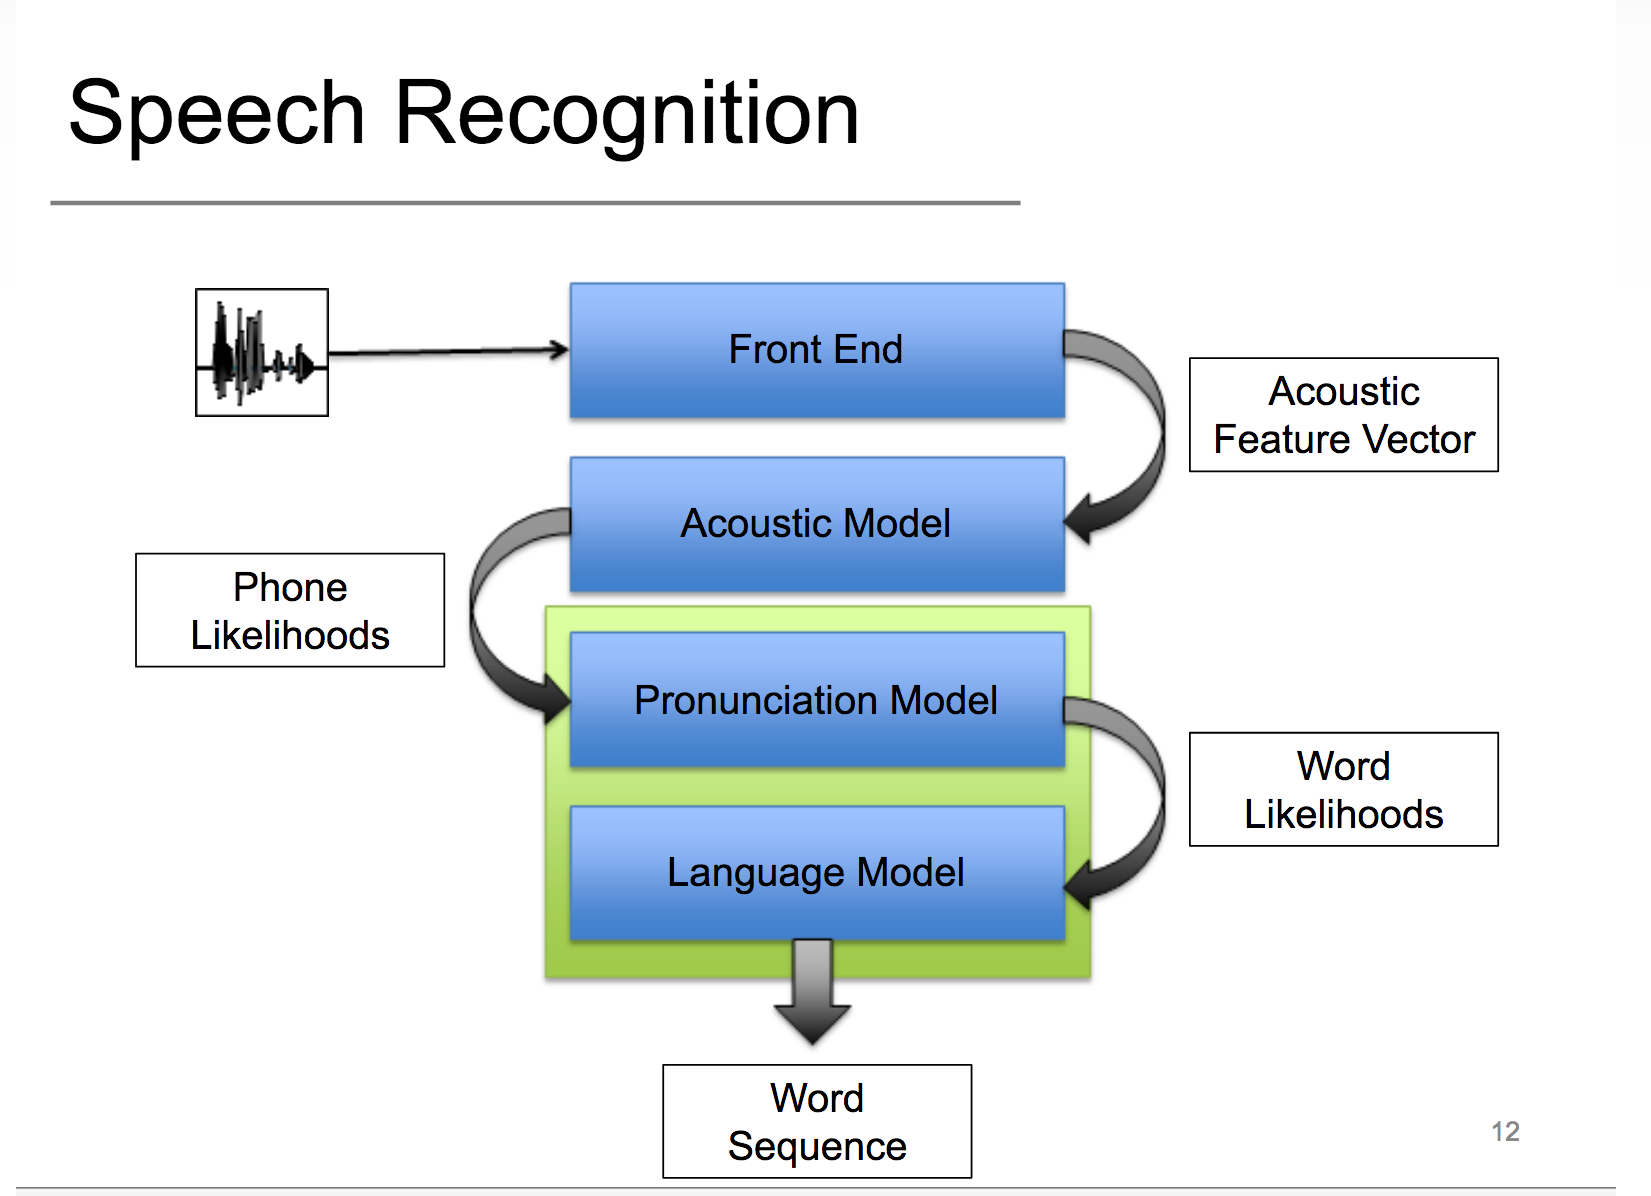
\includegraphics[width=0.9\textwidth]{asr.png}
\\ \tiny source: Andrew Rosenburg's Speech processing lecture.
\end{frame}

\begin{frame}
\frametitle{Building acoustic and pronunciation models}
\begin{itemize}
\item Acoustic model: conversion of speech wave forms in some form of numeric vector indicating properties of that speech sample.
\item Pronunciation model: Mapping sounds to letters, and words.
\item Typically, both of them are put together, and are developed by first collecting hours and hours of recorded speech, creating detailed manual transcriptions for them, and using machine learning to learn to map sounds to words.
\end{itemize}
\end{frame}

\begin{frame}
\frametitle{Building language models}
\begin{itemize}
\item In comparison, getting lots of language data for different languages is not terribly difficult (news papers, wikipedia, movie subtitles etc). 
\item Developing language models (with n-grams, for example) is something we already studied before.
\end{itemize}
\end{frame}

\begin{frame}
\frametitle{Building Pronunciation Models: Issues}
\begin{itemize}
\item Different people pronounce differently - different accents \pause
\item Pronunciation dictionaries: good ones for English, even handle POS variations. But, what about names? what about accents? \pause
\item What about other languages? Where do we get so much of recorded data?? \pause
\item One solution Google came up with: \url{https://research.googleblog.com/2011/03/word-of-mouth-introducing-voice-search.html}
\end{itemize}
\end{frame}

\begin{frame}
\frametitle{Different Forms of ASR}
\begin{itemize}
\item Isolated word recognition (slow speech, each word surrounded by a pause)
\item Read speech recognition (humans talking to machine e.g., dictation)
\item Continuous speech recognition (natural, running speech)
\item Conversational speech recognition (humans talking to each other, noisy environments etc)
\end{itemize}
-these are incrementally harder tasks. (Transcribing a meeting - is it even possible??)
\end{frame}

\begin{frame}
\frametitle{ASR in Real World}
\begin{itemize}
\item All AI-assistants that have spoken language input (Siri, Cortana etc)
\item Google docs support ASR in several languages - did you know that?
\item Dictation tools
\item  \url{swiftscribe.ai} from Baidu.
\end{itemize}
\end{frame}

\begin{frame}
\frametitle{Evaluation of ASR}
\begin{itemize}
\item Word Error Rate
\item Sentence Error Rate
\item In the case of dialog systems involving spoken input: concept error rate
\end{itemize}
\end{frame}

\begin{frame}
\frametitle{Attendance Exercise}
Code-switching refers to people switching between languages while speaking or writing. It is not very common in US, but in multi-lingual societies, it is quite common. What or how do you think ASR systems should be tuned to such scenarios? 

\bigskip \bigskip Next class: Speech Synthesis
\end{frame}

\end{document}
